\section{Factorized Attention-Level Intervention}\label{sec:fali}

\subsection{Architecture-aligned factors}\label{sec:factors}

For one candidate head and one task instance, let $S^{A}$ and $S^{B}$ denote its cached pre-softmax attention-score tensors in the intact and perturbed executions, and let $V^{A}$ and $V^{B}$ denote its corresponding value tensors. Let $q^{\star}$ be the task-relevant query position and $k^{\star}$ the target key position. We use an explicit structural validity mask
\begin{equation}
\mathcal{M}=\{(q,k): q<\ell,\; k\le q\},
\label{eq:valid-mask}
\end{equation}
for a right-padded causal sequence of valid length $\ell$; padding and future positions are structural constants rather than intervention variables. The valid score coordinates are partitioned into
\begin{align}
T &= \{(q^{\star},k^{\star})\}, \\
R &= \{(q^{\star},k)\in\mathcal{M}: k\neq k^{\star}\}, \\
O &= \mathcal{M}\setminus (T\cup R).
\label{eq:tro-partition}
\end{align}
Thus $T$, $R$, and $O$ are pairwise disjoint and cover every structurally valid score coordinate exactly once. When an application specifies multiple target edges, $T$ can be generalized to that prespecified set and $R$ defined as the remaining valid coordinates in the corresponding task-relevant query row(s); the experiments in this paper use one target coordinate per example.

FALI has five binary factors, each taking its value from state $A$ (coded 0) or state $B$ (coded 1):
\begin{itemize}
    \item $T$: task-target attention score(s);
    \item $R$: rival scores in the same task-relevant query row;
    \item $O$: all other structurally valid scores of the candidate head;
    \item $V$: candidate value vectors at all valid source positions;
    \item $C$: surrounding-network context, intact versus perturbed.
\end{itemize}
The first three factors jointly determine the complete candidate attention pattern. $V$ controls the content combined by that pattern. $C$ controls the rest of the model execution outside the explicitly injected candidate state. In particular, $C$ is not defined as a uniquely localized downstream mechanism; it can aggregate differences in other attention heads, MLPs, residual representations, normalization, and upstream or downstream computation.

\subsection{Counterfactual intervention game}\label{sec:game}

Let $(\tau,\rho,\omega,\nu,c)\in\{0,1\}^{5}$ denote one FALI cell. For a binary state index $b$, write $S^{b}=S^{A}$ if $b=0$ and $S^{b}=S^{B}$ if $b=1$, with the analogous convention for $V^{b}$. We construct a hybrid score tensor by taking each coordinate block from its selected endpoint,
\begin{equation}
S_{\tau\rho\omega}
=
\mathbf{1}_{T}\odot S^{\tau}
+\mathbf{1}_{R}\odot S^{\rho}
+\mathbf{1}_{O}\odot S^{\omega},
\label{eq:hybrid-scores}
\end{equation}
with invalid coordinates fixed to the structural attention mask. We then recompute the attention pattern from the hybrid scores,
\begin{equation}
P_{\tau\rho\omega}
=\operatorname{masked\_softmax}(S_{\tau\rho\omega}),
\label{eq:hybrid-pattern}
\end{equation}
and reconstruct the candidate head output using the selected value tensor,
\begin{equation}
z_{\tau\rho\omega\nu}[q]
=\sum_{k}P_{\tau\rho\omega}[q,k]V^{\nu}[k].
\label{eq:hybrid-z}
\end{equation}
The reconstructed $z$ is injected for the candidate head at all valid query positions. This full-output overwrite is important: the live candidate computation is not allowed to leak into a hybrid cell.

Let $F_c[z_h\leftarrow z]$ denote a forward pass in surrounding context $c$, with $c=0$ selecting state $A$ and $c=1$ selecting state $B$, and with the full output of candidate head $h$ replaced by $z$. The FALI utility for a cell is
\begin{equation}
U(\tau,\rho,\omega,\nu,c)
=
 m\!\left(F_c[z_h\leftarrow z_{\tau\rho\omega\nu}]\right)
-
 m\!\left(F_c[z_h\leftarrow 0]\right).
\label{eq:fali-utility}
\end{equation}
The zero-candidate comparison is always evaluated in the same context $c$ as the hybrid injection. FALI therefore contains $2^5=32$ counterfactual cells.

The two complete endpoints recover the effects in Eq.~\ref{eq:context-effect}:
\begin{align}
U(0,0,0,0,0) &= E_A(h), \\
U(1,1,1,1,1) &= E_B(h),
\end{align}
so that
\begin{equation}
\Delta_h
=U(1,1,1,1,1)-U(0,0,0,0,0).
\label{eq:fali-endpoint-identity}
\end{equation}
This endpoint identity is a required implementation invariant, not an approximation in the mathematical definition.

Most mixed cells need not correspond to an activation state encountered during an unmodified forward pass. FALI should therefore be read as an explicit counterfactual/interchange-intervention game. Its attributions are conditional on the chosen endpoint states, target partition, masking semantics, and intervention construction; they are not claims that the model naturally executes five separable causal pathways. Figure~\ref{fig:fali-game} depicts the 32-cell construction.

\begin{figure*}[t]
\centering
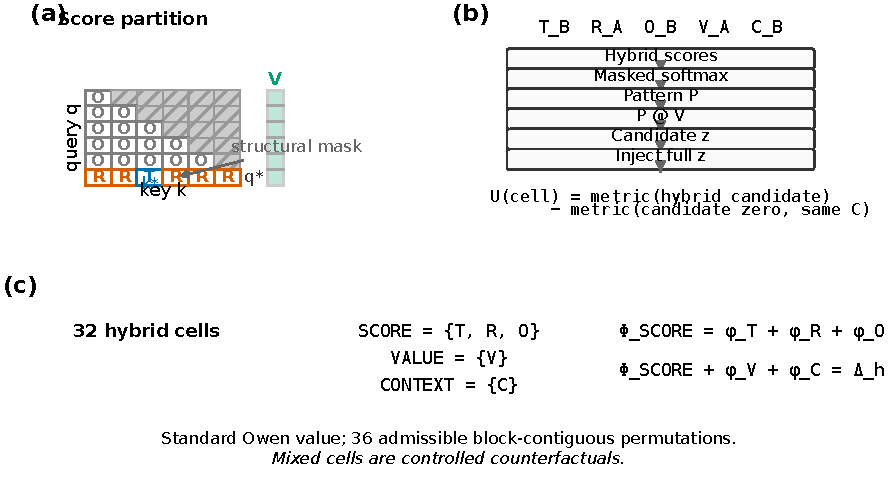
\includegraphics[width=\textwidth]{figures/Fig2.pdf}
\caption{\textbf{FALI constructs a 32-cell counterfactual intervention game for the selected attention head.}
(a) Structurally valid pre-softmax scores are partitioned into the prespecified task-target coordinate(s) $T$, rival scores $R$ in the same task-relevant query row, and all other valid scores $O$; masked coordinates are not players.
(b) Each hybrid cell selects $T,R,O,V,$ and $C$ from the intact or perturbed endpoint, reconstructs the candidate attention pattern and head output, and defines utility relative to a candidate-zero run in the same surrounding context $C$.
(c) All $2^5=32$ hybrid states are evaluated. Standard Owen attribution under $\mathrm{SCORE}=\{T,R,O\}$, $\mathrm{VALUE}=\{V\}$, and $\mathrm{CONTEXT}=\{C\}$ allocates the endpoint change over 36 block-contiguous admissible permutations, satisfying $\sum_i\phi_i=\Delta_h$ and $\Phi_{\mathrm{SCORE}}=\phi_T+\phi_R+\phi_O$.
The mixed cells are controlled counterfactual states, not claims that the model naturally implements five independent causal pathways.}
\label{fig:fali-game}
\end{figure*}


\subsection{Standard Owen attribution and coarse--fine reconciliation}\label{sec:owen}

Let the player set be $N=\{T,R,O,V,C\}$ and associate each coalition $K\subseteq N$ with the cell in which factors in $K$ take their $B$ state and all remaining factors take their $A$ state. This defines the characteristic function
\begin{equation}
v(K)=U(\mathbf{1}_{K}).
\label{eq:characteristic-game}
\end{equation}
Because the score factors are subdivisions of one computational object, whereas value and context are separate coarse factors, we fix the coalition structure
\begin{equation}
\Pi=\{\mathrm{SCORE}=\{T,R,O\},\;\mathrm{VALUE}=\{V\},\;\mathrm{CONTEXT}=\{C\}\}.
\label{eq:owen-partition}
\end{equation}
The partition membership is fixed; the block order is not. We use the standard Owen value, which averages marginal contributions over all permutations in which members of each block remain contiguous \citep{owen1977values}. For this partition there are $3!\times3!=36$ admissible permutations.

For completeness, let $G\in\Pi$ be the block containing player $i$, let $M=|\Pi|=3$, let $\mathcal{B}\subseteq\Pi\setminus\{G\}$ be a subset of predecessor blocks, and let $A_i\subseteq G\setminus\{i\}$ be a subset of predecessor players within $G$. Define $W_{\mathcal{B}}=\bigcup_{H\in\mathcal{B}}H$. The Owen value is
\begin{align}
\phi_i
={}&\sum_{\mathcal{B}\subseteq\Pi\setminus\{G\}}
\frac{|\mathcal{B}|!\,(M-|\mathcal{B}|-1)!}{M!}
\sum_{A_i\subseteq G\setminus\{i\}}
\frac{|A_i|!\,(|G|-|A_i|-1)!}{|G|!} \\
&\quad\times\left[
 v(W_{\mathcal{B}}\cup A_i\cup\{i\})
-v(W_{\mathcal{B}}\cup A_i)
\right].
\label{eq:owen-value}
\end{align}
This is equivalent to averaging sequential marginal contributions over the 36 admissible permutations. We use independent subset-weight and permutation implementations in validation.

The first property needed for interpretation is efficiency:
\begin{equation}
\phi_T+\phi_R+\phi_O+\phi_V+\phi_C
= v(N)-v(\varnothing)
=\Delta_h.
\label{eq:owen-efficiency}
\end{equation}
The attributions therefore allocate the entire endpoint change in causal usefulness, including interaction effects, under the specified game. They should not be interpreted as pure direct effects.

The second property gives the coarse--fine bridge. Define the quotient game on the three meta-players by
\begin{equation}
q(\mathcal{K})=v\!\left(\bigcup_{G\in\mathcal{K}}G\right),
\qquad \mathcal{K}\subseteq\Pi.
\label{eq:quotient-game}
\end{equation}
Standard Owen group consistency gives
\begin{align}
\Phi_{\mathrm{SCORE}}
&=\phi_T+\phi_R+\phi_O
=\operatorname{Shapley}_{q}(\mathrm{SCORE}), \\
\phi_V&=\operatorname{Shapley}_{q}(\mathrm{VALUE}), \\
\phi_C&=\operatorname{Shapley}_{q}(\mathrm{CONTEXT}).
\label{eq:quotient-consistency}
\end{align}
When the whole SCORE block switches together, its hybrid scores reproduce the complete $A$ or $B$ candidate pattern. The quotient SCORE/V/C game therefore matches the earlier pattern/value/context intervention game at the corresponding cells; this numerical bridge is tested explicitly in Section~\ref{sec:implementation-validation}. The purpose of Owen attribution here is not mathematical novelty but consistency between a coarse score/value/context explanation and the finer $T/R/O$ explanation inside SCORE.

Finally, the historical two-factor attention-probability version of FALI is nested as a special case rather than identified with the present causal attributions. If the utility is changed from output-grounded usefulness to target attention probability, $O$, $V$, and $C$ are held fixed, and only $T$ and $R$ vary, Eq.~\ref{eq:owen-value} reduces to the ordinary two-player Shapley decomposition of target-score versus competing-score changes. The present method changes both the intervention scope and, crucially, the quantity being explained.
